\documentclass{beamer}
\usetheme{metropolis}
\usepackage{graphicx}
\usepackage{subcaption}
\usepackage{hyperref}
\usepackage{tcolorbox}
\title{Algebra-Based Physics-1: Mechanics (PHYS135A-01): Week 9}
\date{October 30th - November 3rd, 2017}
\author{Jordan Hanson}
\institute{Whittier College Department of Physics and Astronomy}

\begin{document}
\maketitle

\section{Week 8 Review}

\begin{frame}{Week 8 Summary}
\begin{enumerate}
\item Definition of \alert{\textbf{momentum}}
\item \alert{\textbf{\textit{Conservation of momentum}}}
\begin{itemize}
\item The proof and the assumptions
\item Examples
\end{itemize}
\item \alert{\textbf{\textit{Classification of collisions}}}
\begin{itemize}
\item Elastic
\item Inelastic
\item $1 \rightarrow 1$, $1 \rightarrow n$, $n \rightarrow 1$, $n \rightarrow n$
\item \textbf{Lab activity}
\end{itemize}
\item \textbf{Momentum in multiple dimensions}
\item \textbf{Center of mass}
\begin{itemize}
\item Derivation of $\vec{F}_{\rm Net} = \frac{d\vec{P}_{\rm CM}}{dt}$
\item Center of mass motion
\end{itemize}
\end{enumerate}
\end{frame}

\section{Week 8 Review Problems}

\begin{frame}{Week 8 Review Problem}
\small Imagine a space shuttle launch.  Rocket propellant is ignited and blasted out of the solid rocket boosters (SRBs).  Which of the following is true of the shuttle-propellant system? \\
\begin{itemize}
\item A: The exhaust pushes on the against the ground, and by Newton's 3rd Law, the ground pushes on the rocket, and the rocket accelerates upward.
\item B: The exhaust pushes on the air, and by Newton's 3rd Law, the air pushes on the rocket and it accelerates upward.
\item C: The momentum of the rocket increases because the ejected mass results in a force on the rocket via Newton's 3rd Law
\item D: The rocket pushes out the exhaust, and by Newton's 3rd Law, the exhaust pushes on the rocket
\end{itemize}
\end{frame}

\begin{frame}{Week 8 Review Problem}
\small An Apollo class spacecraft has made it far enough to the Moon that we can neglect Earth's gravity.  It is comprised of two pieces of equal mass, and the whole system is moving at speed $v$.  If one piece is launched backward such that it remains stationary, what is the new speed of the craft?
\begin{itemize}
\item A: $v$
\item B: $2v$
\item C: $4v$
\item D: $0$
\end{itemize}
\end{frame}

\section{Week 9 Summary}

\begin{frame}{Week 9 Summary}
\textit{We are concluding with chapter 10, regarding angular momentum. Please read chapter 10.}
\begin{enumerate}
\item Review of \textbf{angular motion}
\begin{itemize}
\item Angular velocity and acceleration
\item \textit{Torque}
\end{itemize}
\item \alert{The moments of inertia}
\item Newton's 2nd Law, rotational case
\item Energy of Rotating Objects
\begin{itemize}
\item \textbf{Conservation of energy, revisited}
\item Rotational kinetic energy
\item Examples of work
\end{itemize}
\item \textbf{\alert{Conservation of angular momentum}}
\item Begin review of all chapters
\end{enumerate}
\end{frame}

\section{Review of Angular Motion}

\begin{frame}{Review of Angular Motion}
\begin{columns}[T]
\begin{column}{0.5\textwidth}
\begin{figure}
\centering
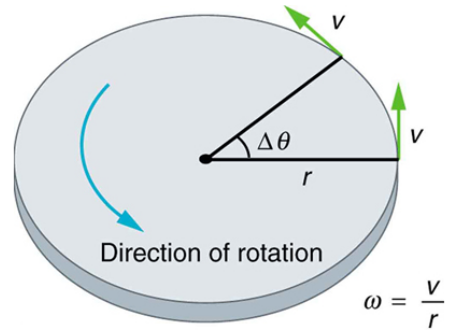
\includegraphics[width=0.6\textwidth]{figures/angle.png}
\caption{\label{fig:angle} From the definition of a radian we may derive angular velocity and acceleration.}
\end{figure}
\end{column}
\begin{column}{0.5\textwidth}
\begin{figure}
\centering
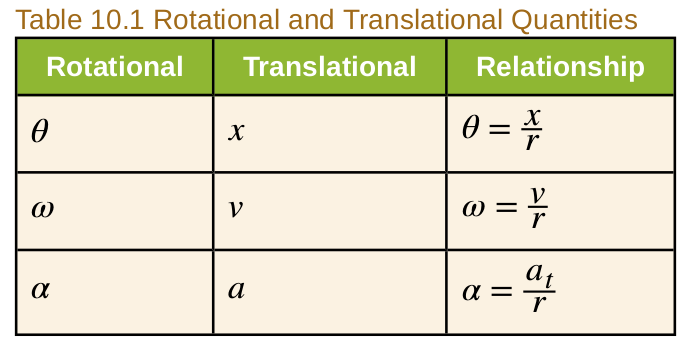
\includegraphics[width=0.89\textwidth]{figures/angle2.png}
\caption{\label{fig:angle2} Review of angular kinematic quantities.}
\end{figure}
\end{column}
\end{columns}
\end{frame}

\begin{frame}{Review of Angular Motion}
\begin{columns}[T]
\begin{column}{0.5\textwidth}
\begin{figure}
\centering
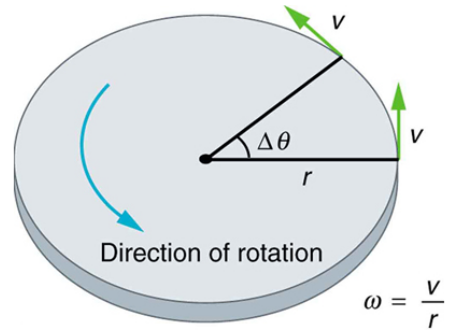
\includegraphics[width=0.6\textwidth]{figures/angle.png}
\caption{\label{fig:angle3} From the definition of a radian we may derive angular velocity and acceleration.}
\end{figure}
\end{column}
\begin{column}{0.5\textwidth}
\begin{figure}
\centering
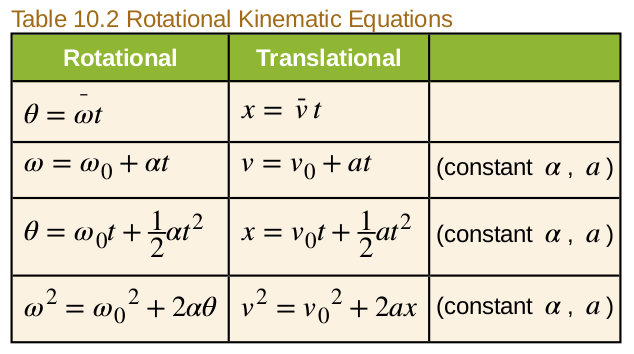
\includegraphics[width=0.89\textwidth]{figures/angle3.png}
\caption{\label{fig:angle4} Review of angular kinematic quantities.}
\end{figure}
\end{column}
\end{columns}
\end{frame}

\begin{frame}{Review of Angular Motion}
A fishing rod is comprised of a pole and a reel for the fishing line.  The reel of a particular model has a radius of 5 cm, and a man casts the line, letting out 5 meters in 1 second.  What is the angular velocity of the reel?
\begin{itemize}
\item A: 5 radians per second
\item B: 10 radians per second
\item C: 50 radians per second
\item D: 100 radians per second
\end{itemize}
\end{frame}

\begin{frame}{Review of Angular Motion}
\begin{columns}[T]
\begin{column}{0.5\textwidth}
\begin{figure}
\centering
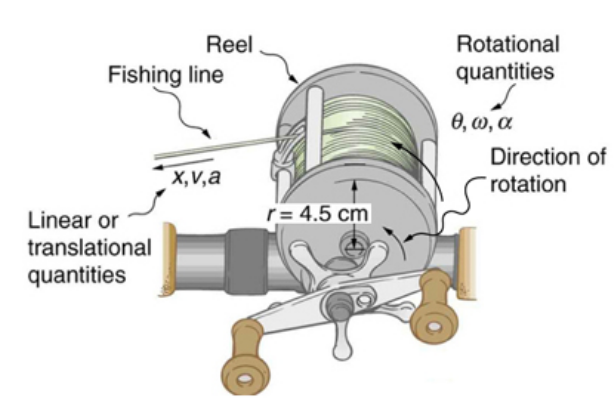
\includegraphics[width=\textwidth]{figures/angle4.png}
\caption{\label{fig:angle5} From the definition of a radian we may derive angular velocity and acceleration.}
\end{figure}
\end{column}
\begin{column}{0.5\textwidth}
If the man catches a fish on the line, the line will have tension.  \textit{What about the reel?}  There is tension on the reel, but not ``at the center.'' \\ \vspace{0.5cm}
\textbf{The concept of torque} is that a force leads to \textit{rotational} rather than \textit{linear} motion.  \alert{Would it be harder to reel in the fish with a reel of larger or smaller radius?}
\end{column}
\end{columns}
\end{frame}

\begin{frame}{Review of Angular Motion}
Let \textit{torque} be defined as the \textbf{cross-product} of a force, $F$ and a moment-arm, $r$:
\begin{equation}
\vec{\tau} = \vec{r} \times \vec{F}
\end{equation}
\textbf{Cross-product}: a new way of multiplying vectors: $\hat{i} \times \hat{j} = \hat{k}$, $\hat{k} \times \hat{i} = \hat{j}$, $\hat{j} \times \hat{k} = \hat{i}$.  See the pattern?  (There's the \textbf{right-hand rule}).  Although torque is a vector, presently we are concerned with the magnitude of torque:
\begin{equation}
\tau = r F \sin\theta
\end{equation}
The angle $\theta$ is between the force and the moment arm.  \textbf{The units are: N m}.  What other quantity has these units?
\end{frame}

\begin{frame}{Review of Angular Motion}
If a 1 kg fish is hanging from a fishing pole that is 1.5 meters long and held horizontally, what is the torque?
\begin{itemize}
\item A: 15 N m
\item B: 10 N m
\item C: 1.5 N m
\item D: 10 N
\end{itemize}
\end{frame}

\begin{frame}{Review of Angular Motion}
If a 1 kg fish is hanging from a fishing pole that is 1.5 meters long and held vertically, what is the torque?
\begin{itemize}
\item A: 15 N m
\item B: 1.5 N m
\item C: 0 N m
\item D: 10 N
\end{itemize}
\end{frame}

\begin{frame}{Review of Angular Motion}
Previous two questions:
\begin{equation}
\tau = r F \sin\theta
\end{equation}
The angle $\theta$ is between the force and the moment arm, so if $\theta = 0$ then there is no torque, and if $\theta = 90^{\circ}$ then torque maximizes at $\tau = rF$.
\end{frame}

\section{Moments of Inertia}

\begin{frame}{Moments of Inertia}
Starting with Newton's 2nd law, we may reveal something called the \textbf{moment of inertia}, through the concept of torque:
\begin{align}
F &= ma \\
a &= r\alpha \\
F &= mr\alpha \\
rF &= mr^2\alpha \\
\tau &= (m r^2) \alpha \\
I &= mr^2 \\
\tau &= I \alpha
\end{align}
\textit{Newton's 2nd Law in rotational form} is that torque is equal to the \textit{moment of inertia}, $I$, times the angular acceleration $\alpha$.
\end{frame}

\begin{frame}{Moments of Inertia}
\textit{Newton's 2nd Law in rotational form} is that torque is equal to the \textit{moment of inertia}, $I$, times the angular acceleration $\alpha$.  \alert{The moment of inertia describes spatial distribution of mass}.  \\ \vspace{0.5cm} Although the formula $I = mr^2$ only applies to a single piece of matter a distance $r$ along the moment-arm, we may derive the moment of inertia for \textit{any rigid body} through the techniques of calculus.
\end{frame}

\begin{frame}{Moments of Inertia}
\begin{figure}
\centering
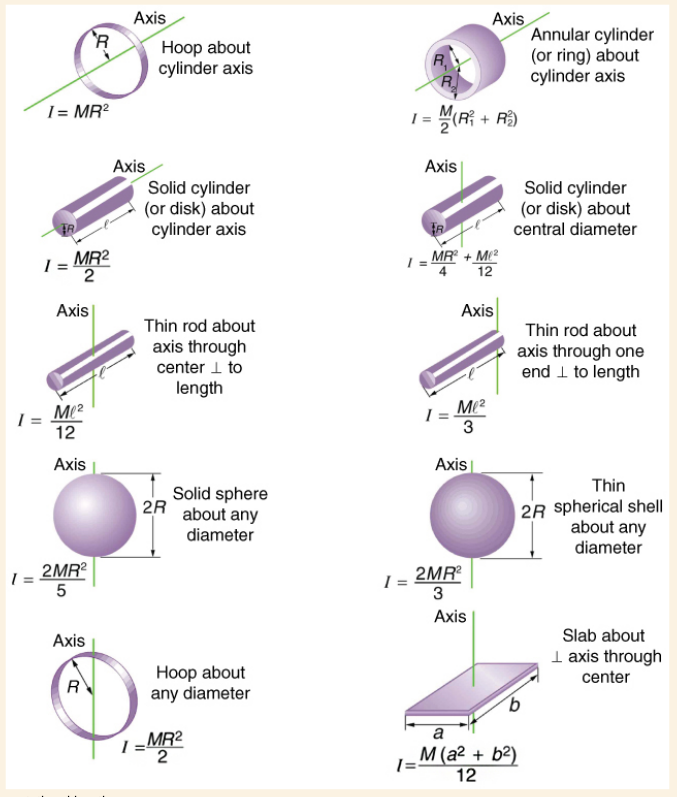
\includegraphics[width=0.53\textwidth]{figures/moment.png}
\caption{\label{fig:moment} Moments of inertia about different axes of rotation.}
\end{figure}
\end{frame}

\begin{frame}{Review of Angular Motion}
Basketball players are taught how to shoot a jump shot with a \textit{backspin}.  The moment of inertia of a basketball is like that of a thin spherical shell: $I = \frac{2}{3}MR^2$, where $M$ is the mass of the basketball and $R$ is the radius.  If a basketball has a 10 cm radius, and a mass of 0.6 kg, what is the moment of inertia?
\begin{itemize}
\item A: $4\times 10^{-2}$ kg m$^2$
\item B: $4\times 10^{-3}$ kg m$^2$
\item C: $4\times 10^{-1}$ kg m$^2$
\item D: $4\times 10^{-3}$ kg
\end{itemize}
\end{frame}

\begin{frame}{Review of Angular Motion}
Basketball players are taught how to shoot a jump shot with a \textit{backspin}.  The moment of inertia of a basketball is $4\times 10^{-3}$ kg m$^2$.  What torque is required to make the ball go from 0 radians/sec to $10\pi$ radians/sec in 0.1 second? (Angle between force and moment-arm: 90 deg).
\begin{itemize}
\item A: $4\times 10^{-2}$ kg m$^2$
\item B: $\frac{2\pi}{500}$ N m
\item C: $\frac{2\pi}{5}$ N
\item D: $\frac{2\pi}{5}$ N m
\end{itemize}
\end{frame}

\begin{frame}{Review of Angular Motion}
Basketball players are taught how to shoot a jump shot with a \textit{backspin}.  If the radius of the ball were twice as large, by what factor would the torque need to increase to produce the same angular acceleration?
\begin{itemize}
\item A: $2$
\item B: $4$
\item C: $2\sin\theta$
\item D: No change
\end{itemize}
\end{frame}

\section{Conservation of Energy, Revisited}

\begin{frame}{Conservation of Energy}
In the exact same fashion as the linear case, we can show that work done on a rotating system increases the \textit{rotational kinetic energy}:
\begin{equation}
W = \frac{1}{2}I\omega^2 - \frac{1}{2}I\omega_{\rm 0}^2 \label{eq:eq1}
\end{equation}
In Eq. \ref{eq:eq1}, the rotational kinetic energy is $KE_{\rm rot} = \frac{1}{2}I\omega^2$.  The moment of inertia takes the place of mass, and the angular velocity takes the place of linear velocity.
\end{frame}

\begin{frame}{Conservation of Energy}
The presence of rotational kinetic energy in a system requires us to revisit the conservation of energy.  One way to state this principal is to assume all potential energy is converted to kinetic energy: 
\begin{equation}
\boxed{PE_{\rm i} = KE_{\rm trans} + KE_{\rm rot}}
\end{equation}
\end{frame}

\begin{frame}{Conservation of Energy}
Return to the basketball with \textit{backspin} scenario.  Suppose the basketball is shot with some known speed, angle, and backspin.  The ball swooshes through the hoop.  If the same player shoots the same shot from the same place, but increases the backspin, which of the following is true?
\begin{itemize}
\item A: The shot will fall short
\item B: The shot will go long and hit the backboard
\item C: The shot will still go in
\item D: The shot will still go in, but take more time
\end{itemize}
\end{frame}

\begin{frame}{Conservation of Energy}
Suppose two basketballs with different radii roll down a driveway.  The moment of inertia for this shape is $I = \frac{2}{3}MR^2$ if $M$ is the mass and $R$ is the radius.  Which of the following is true?
\begin{itemize}
\item A: The basketball with the larger radius will reach the bottom of the driveway first
\item B: The basketball with the smaller radius will reach the bottom of the driveway first
\item C: The basketballs will reach the bottom of the driveway at the same time
\item D: The basketball with the larger mass
\end{itemize}
\end{frame}

\section{An Example of Work}

\begin{frame}{An Example of Work}
\small
A \textbf{grindstone} is used to sharpen knives and cutlery.  A grindstone is a disk spinning about the natural axis, with $I = \frac{1}{2}MR^2$.  Work done on the grindstone to sap its energy would be $W = \tau\theta$, where $\tau$ is the torque and $\theta$ is angular displacement.  \\ \vspace{0.5cm}
Newton's 2nd Law gives $\tau = I\alpha$, so $W = \frac{1}{2}\alpha\theta MR^2$. \\ \vspace{0.5cm}
\end{frame}

\begin{frame}{Conservation of Energy}
Suppose we press our pocketknife to a 20 kg grindstone with radius 10 cm, that is spinning at 10 radians per second (no net external force).  If we press really hard the grindstone comes to a stop after 10 seconds.  How much energy went into sharpening the knife? \\ \vspace{1cm}
\textbf{Solve in groups at the boards.}
\end{frame}

\section{Conservation of Angular Momentum}

\begin{frame}{Conservation of Angular Momentum}
The running theme is that for every \textit{linear} idea we developed, there is a corresponding \textit{rotational} idea.  Just as we found that the momentum $\vec{p} = m\vec{v}$ is a conserved quantity under two conditions, so is the \textbf{angular momentum}:
\begin{equation}
L = I\omega
\end{equation}
The conditions are what you would expect:
\begin{itemize}
\item The moment of inertia does not change.
\item No net external torque.
\end{itemize}
\end{frame}

\begin{frame}{Conservation of Angular Momentum}
\small
Shouldn't angular momentum be a vector, since linear momentum is a vector?
\begin{equation}
\vec{L} = I\vec{\omega}
\end{equation}
But what is $\vec{\omega}$?  We can simply define it as
\begin{equation}
r^2 \vec{\omega} = \vec{r} \times \vec{v}
\end{equation}
That is, it's proportional to the cross-product of the moment-arm and the linear velocity of a rotating system.  Think about the sine function that goes with the cross-product: if the angle betwee $r$ and $v$ is zero then $\vec{\omega}$ should be zero because the system is not rotating.
\end{frame}

\begin{frame}{Conservation of Angular Momentum}
\small
If we substitute the definition of $\vec{\omega}$ into $\vec{L} = I\vec{\omega}$, then we find for a particle of mass $m$ with $I = mr^2$
\begin{equation}
\vec{L} = \vec{r} \times \vec{p}
\end{equation}
Look at the time-dependence, though: if $r$ is constant in time, then the change in $\vec{L}$ depends only on $\Delta\vec{p}/\Delta t$.  Under certain conditions $\Delta\vec{p}/\Delta t = 0$ (\textbf{no net external forces, mass is constant}).  \alert{These imply no net torque, and moment of inertia is constant for \textit{rigid bodies}.}
\begin{equation}
\boxed{\frac{d\vec{L}}{dt} = 0}
\end{equation}
Angular momentum is conserved.
\end{frame}

\begin{frame}{Conservation of Angular Momentum}
\textbf{Demonstration of angular momentum conservation:} spin the professor.
\end{frame}

\begin{frame}{Conservation of Angular Momentum}
\begin{figure}
\centering
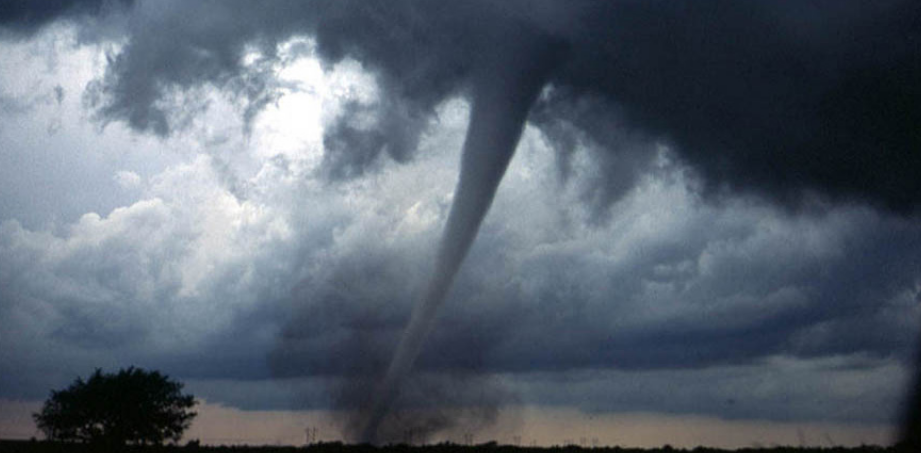
\includegraphics[width=\textwidth]{figures/twister.png}
\caption{\label{fig:twist}  I was born in Oklahoma, where angular momentum is a part of life.}
\end{figure}
\end{frame}

\begin{frame}{Conservation of Angular Momentum}
Angular momentum in the movies:
\url{https://www.youtube.com/watch?v=c4tPQYNpW9k}
\end{frame}

\begin{frame}{Conservation of Angular Momentum}
\small
I read a story once that some NASA astronauts in the early days of the space program realized a leak was causing their overall craft to begin to spin, but that they could detach that part of the spacecraft that was leaking.  Imagine the craft as two pieces, both cylinders, attached at the bases, with one leaking.  If the whole thing is spinning, what happened when the astronauts separated the cylinders?
\begin{itemize}
\item A: Each cylinder began to spin slower, but the leaky one sped up.
\item B: Each cylinder spun at the same rate, but the leaky one sped up.
\item C: Each cylinder began to spin faster, and the leaky one sped up.
\item D: The cylinder without the leak stopped spinning, and the leaky one continued to spin faster.
\end{itemize}
\end{frame}

\begin{frame}{Beyond Classical Physics}
\begin{figure}
\centering
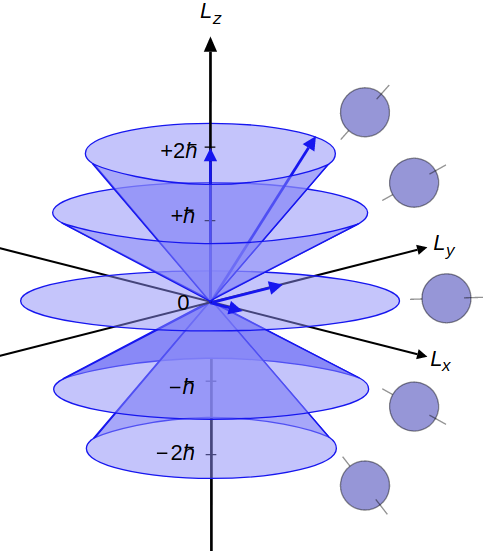
\includegraphics[width=0.5\textwidth]{figures/L.png}
\caption{\label{fig:L}  Quantization of angular momentum in quantum mechanics, and Planck's constant in quantum mechanics...}
\end{figure}
\end{frame}

\section{Conclusion}

\begin{frame}{Week 9 Summary}
\textit{We are concluding with chapter 10, regarding angular momentum. Please read chapter 10.}
\begin{enumerate}
\item Review of \textbf{angular motion}
\begin{itemize}
\item Angular velocity and acceleration
\item \textit{Torque}
\end{itemize}
\item \alert{The moments of inertia}
\item Newton's 2nd Law, rotational case
\item Energy of Rotating Objects
\begin{itemize}
\item \textbf{Conservation of energy, revisited}
\item Rotational kinetic energy
\item Examples of work
\end{itemize}
\item \textbf{\alert{Conservation of angular momentum}}
\item Begin review of all chapters
\end{enumerate}
\end{frame}

\begin{frame}{Final Presentations}
\textit{This is a sketch of what should be contained in the final presentations of your science projects.}
\begin{enumerate}
\item Introduction of the concepts, the goal
\item Diagram or picture of the experiment, expressing how the measurement is performed
\item Present the data, and any associated systematic errors
\item Conclusion, compare to hypothesis
\end{enumerate}
\textbf{Final presentations will be on December 6th, during class time.  Please bring them on a USB memory stick, or be able to access them online via a tool like Dropbox.  Let me know if you need a USB memory stick.}
\end{frame}

\section{Answers}

\begin{frame}{Answers}
\small
\begin{columns}[T]
\begin{column}{0.5\textwidth}
\begin{itemize}
\item C and D
\item $2v$
\item 100 radians per second
\item 15 N m
\item 0 N m
\item $4\times 10^{-3}$ kg m$^2$
\item $\frac{2\pi}{5}$ N m
\item $2$
\item The shot will fall short
\item The basketball with the smaller radius will reach the bottom of the driveway first
\end{itemize}
\end{column}
\begin{column}{0.5\textwidth}
\begin{itemize}
\item Each cylinder began to spin faster, and the leaky one sped up.
\end{itemize}
\end{column}
\end{columns}
\end{frame}

\end{document}
